\newpage
\section{Gestione domande}
Selezionata la voce \textit{Gestione delle domande} dal menù a sinistra il sistema visualizza la seguente pagina, dalla quale un utente può gestire le proprie domande:

\label{GestioneDomande}
\begin{figure}[ht]
	\centering
	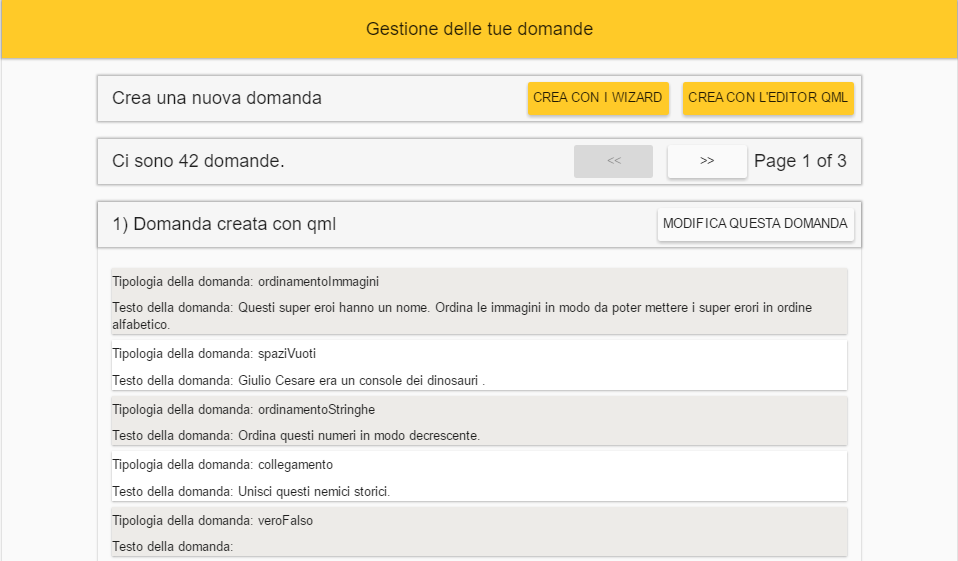
\includegraphics[scale=0.45]{img/gestione_domande.png}
	\caption{Gestione delle domande}
\end{figure}
\FloatBarrier

All'interno della pagina è visibile l'elenco di tutte le domande create, con la possibilità di modificarle. E' possibile poi creare una nuova domanda attraverso due differenti funzionalità: \textit{CREA CON I WIZARD} e \textit{CREA CON L'EDITOR QML}.

\newpage
\subsection{Crea domanda tramite QML}
Selezionata la voce \textit{CREA CON L'EDITOR QML} il sistema porta l'utente alla seguente pagina, nella quale potrà creare una nuova domanda digitando codice \textit{QML\ped{G}} (si veda Appendice A) direttamente nell'editor di testo presentato:

\label{CreaDomandaQML}
\begin{figure}[ht]
	\centering
	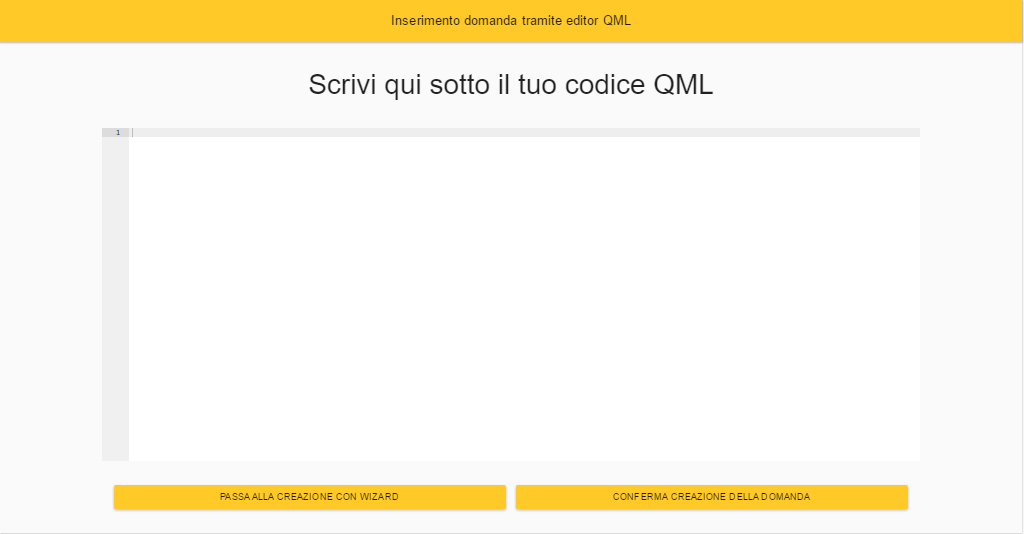
\includegraphics[scale=0.40]{img/domanda_qml.png}
	\caption{Crea domanda tramite QML}
\end{figure}
\FloatBarrier

Digitato il corretto codice della domanda nell'editor, sarà possibile cliccare il pulsante \textit{CONFERMA CREAZIONE DELLA DOMANDA} per creare la domanda. Essa sarà così visibile all'interno dell'elenco presentato nella pagina \textit{Gestione domande}.